\documentclass[12pt,a4paper]{article}

\usepackage[T1]{fontenc}
\usepackage[polish]{babel}
\usepackage[utf8]{inputenc}
\usepackage{lmodern}
\selectlanguage{polish}
\usepackage{graphicx}
\usepackage{biblatex}
\usepackage{csquotes}
\addbibresource{bib.bib}

\begin{document}


\nocite{*}

\pagenumbering{gobble}
\clearpage
\begin{figure}[h]
\centering

\includegraphics{media/ps-logo.png}
\end{figure}
\hspace{3cm}
\begin{center}Dokumentacja projektowa\end{center}
\begin{center}MLA 2021/2022\end{center}
\hspace{3cm}
\begin{center}\large\textbf{Aplikacje uczenia maszynowego \\w systemach interakcji człowiek-maszyna}\end{center}
\hspace{7cm}
\begin{flushright}Kierunek: Informatyka
\end{flushright}
\begin{flushright}Członkowie zespołu:
\par
\textit{Dawid Bitner}
\par
\textit{Daniel Broczkowski}
\par
\textit{Damian Kwaśniok}
\end{flushright}
\vfill
\begin{center}Gliwice, 2021/2022\end{center}

\newpage
\pagenumbering{arabic}
\tableofcontents

\newpage
\section{Wprowadzenie}

\subsection{Cel projektu}
Celem projektu było wykonanie systemu opierającego się o interakcję człowiek-komputer. Zespół projektowy postanowił zaimplementować aplikację rozpoznającą, czy osoba stająca przed kamerą ma założoną maseczkę na twarzy. Projekt nosi nazwę ,,face mask detector''. Głównym celem projektu było stworzenie użytecznej aplikacji mogącej mieć zastosowanie w obszarze przestrzeni publicznej (uczelnie, urzędy, inne placówki publiczne) jak i mogącej być wykorzystywanej przez podmioty prywatne - projekt miał za zadanie pokazać w jaki sposób interakcja człowiek-komputer może być wykorzystywana w codziennym życiu. 

\subsection{Zespół projektowy}
Dawid Bitner    :: Deweloper   :: Opracowanie obszaru ML i HCI, implementacja projektu końcowego.\newline
Daniel Broczkowski    :: Deweloper   :: Opracowanie obszaru ML i HCI, implementacja projektu końcowego.\newline
Damian Kwaśniok    :: Deweloper   :: Opracowanie obszaru ML i HCI, implementacja projektu końcowego.

\newpage

\section{Założenia projektowe}
Do głównych zależeń projektowych określonych przez zespół implementujący rozwiązanie można zaliczyć m.in.:
\begin{itemize}
\item uniwersalność
\item skalowalność
\item możliwość ulepszeń
\item wykorzystanie \textit{Machine Learningu}
\item oparcie o interakcję człowiek-komputer
\end{itemize}

Zdaniem zespołu odpowiedzialnego za projekt wszystkie założenia zostały spełnione. System detekcji maski na twarzy można uruchamiać na urządzeniach z różnymi systemami operacyjnymi np.; \textit{Microsoft Windows}, \textit{Linux}. Projekt może być uruchomiony na każdym środowisku, na którym został zainstalowany interpreter \textit{Python 3} wraz z bibliotekami.

Program jest skalowalny oraz podatny na ulepszenia, może on być ciągle udoskonalany poprzez dodanie dodatkowych opcji w przyszłości np.: oprócz rozpoznawania maseczki na twarzy dodanie rozpoznawanie osoby przed kamerą. Szczególnie przydatne jeżeli oprócz weryfikacji noszenia maski potrzeba również weryfikować osobę przed kamerą, np.: czy jest nauczycielem akademickim, pracownikiem itp.

Program został przeszkolony w celu detekcji maski na twarzy za pomocą uczenia maszynowego. Zachodzi również interakcja człowiek-komputer, czy też człowiek-maszyna. Osoba podchodzi do kamery, oprogramowanie weryfikuje czy ma założoną maseczkę, następnie na podstawie wyniku działania algorytmu można podjąć decyzję co do wyniku.
\newpage

\section{Implementacja}
Projekt został zaimplementowany w oparciu o język programowania \textit{Python}. wykorzystane zostały składowe takich bibliotek jak \textit{TensorFlow}, \textit{Keras}, \textit{Numpy}.

W pierwszej kolejności zostały wybrany zbiór danych do przetrenowania. Trzeba podkreślić, że wybrany zbiór nie jest idealny, zostały w nim użyte tylko chirurgiczne maseczki o jasnej kolorystyce, oraz w niektórych przypadkach zostały one doklejone do zdjęcia za pomocą obróbki graficznej. Z tego też powodu, co zostanie przedstawione w kolejnym rozdziale system nie do końca poprawnie rozpoznaje sytuację w której osoba przed kamerą ma założoną ciemną maseczkę. Zdjęcia do treningu i testów zostały podzielone na dwie grupy: z maseczką i bez maseczki.
\begin{figure}[h!]
    \centering
    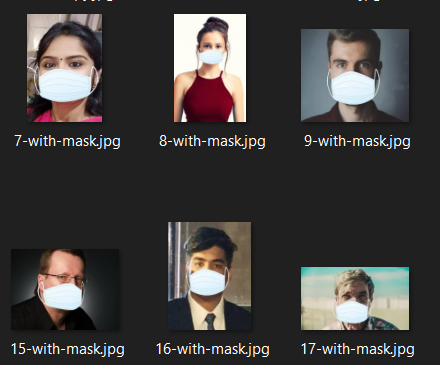
\includegraphics[scale = 1]{media/mask.png}
    \caption{Część zbioru danych do treningu - z maseczką}
    \label{fig:Rysunek1}
\end{figure}
\newpage
Następnie został stworzony skrypt z siecią neuronową - 8 warstwową, która trenuje i testuje program. 
\begin{figure}[h!]
    \centering
    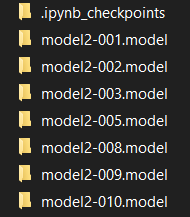
\includegraphics[scale = 1]{media/modele.png}
    \caption{Modele wynikowe}
    \label{fig:Rysunek1}
\end{figure}
W ostatniej kolejności został napisany skrypt integrujący kamerę w urządzeniu z systemem wykrywani twarzy. Wyniki działania widoczne są w kolejnym rozdziale.

\section{Badania}
Zespół projektowy podczas wykonywania projektu sugerował się najnowszymi trendami w dziedzinie \textit{Machine Leariningu}, stworzona sieć działa poprawnie, nie obciąża mocno systemu operacyjnego, oraz na wybranym zbiorze danych działa w naszej opinii dosyć szybko. W teorii sytsem powinien wykrywać przede wszystkim głowę osoby za pomocą klasyfikatora twarzy \textit{haarcascade\_frontalface\_default} - który w pliku \textit{.xml} zawiera zbiór koordynatów opracowany przez firmę \textit{Intel} na licencji \textit{Open Source} - o czym informuje w komentarzu w pliku. Dodatkowo system sprawdza to, czy badany osobnik ma założoną maseczkę, czy też jej nie ma. W praktyce zadanie to nie zawsze jest spełniane w stu procentach, co przedstawione jest na poniższych przykładach.

\begin{figure}[h!]
    \centering
    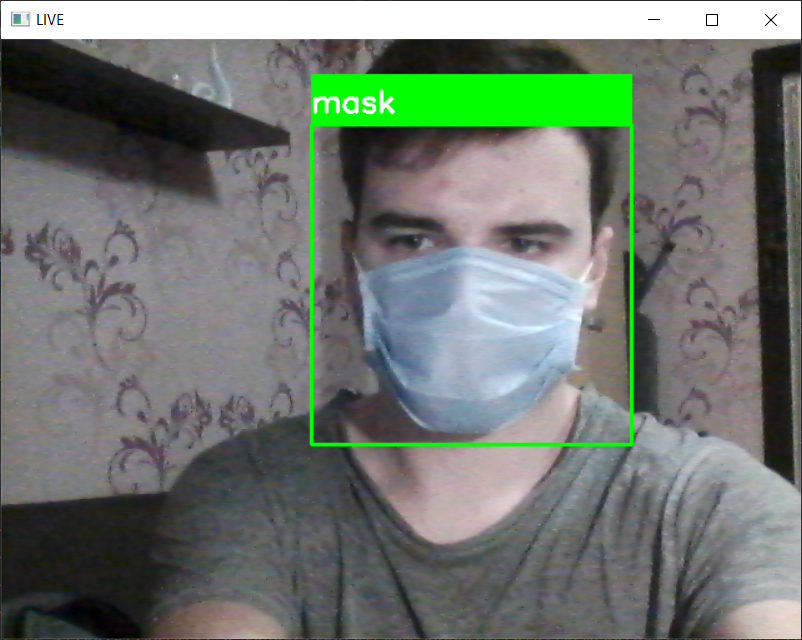
\includegraphics[scale = 0.38]{media/true_z.png}
    \caption{Prawidłowo wykryta twarz z maseczką.}
    \label{fig:Rysunek1}
\end{figure}

\begin{figure}[h!]
    \centering
    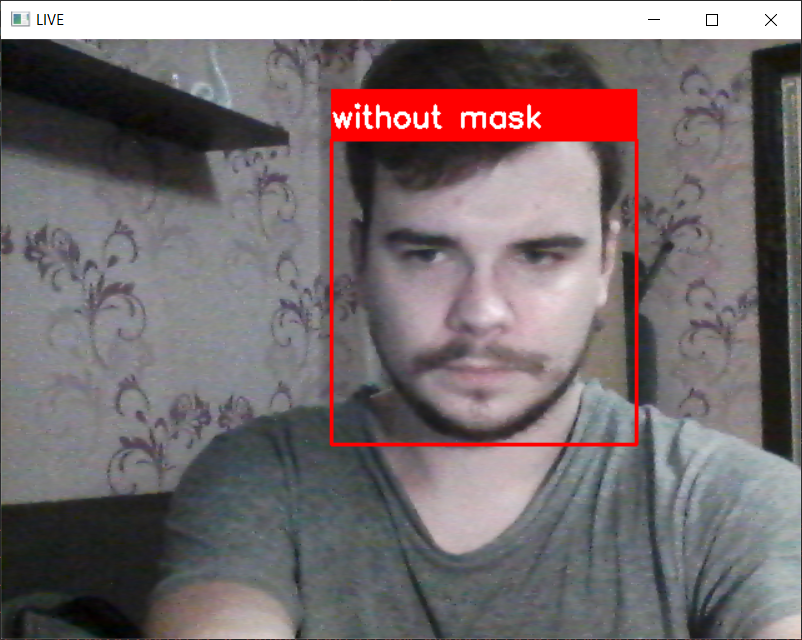
\includegraphics[scale = 0.38]{media/false_bez.png}
    \caption{Prawidłowo wykryta twarz bez maseczki}
    \label{fig:Rysunek2}
\end{figure}
\newpage
Pierwsze dwa przypadki zostały prawidłowo rozpoznane. Jest to w głównej mierze zasługa dwóch czynników. Pierwszy z nich to dobre oświetlenie - badana twarz jest jasna, a jej kontury kontrastują z tłem. Drugim czynnikiem jest sam zbiór treningowy, który nie jest takiej jakości, jakiej zespół projektowy by sobie życzył. Nierzadko maseczki zostały doklejone do zdjęć w programach graficznych, przez co brakuje normalizacji sceny zdjęcia i maseczka wyraźnie kontrastuje na tle reszty głowy (warto zauważyć, iż w omawianym przypadku użyto maseczki o błękitnym kolorze).

\newpage

\section{Podsumowanie i wnioski}

\begin{itemize}
\item \textit{Podsumowanie}

System cechuje wysoką skutecznością. Biorąc pod uwagę zbiory testowe i treningowe wynosi ona ok. \textit{92\%} biorąc pod uwagę wymóg testu w jasnej maseczce. Naszym zdaniem - jak na zbiór danych którym został przetrenowany, działa bardzo dobrze. System również poprawnie wykrywa istnienie twarzy. 

\item \textit{Wnioski}

System jest prosty, łatwy do uruchomienia na różnych środowiskach, naszym zdaniem do tego powinno dążyć nowoczesne oprogramowanie. System niepoprawnie wykrywa ciemne maseczki, kolejna iteracja szkolenia systemu powinna przebiegać na nieco bardziej zróżnicowanych obrazach testowych (różnokolorowe maski). Z pewnością jest to najważniejszy obszar do przepracowania w tej implementacji. 

\end{itemize}

\newpage
\section{Spis literatury}

\printbibliography[heading=none] 

\end{document}
